\documentclass[a4paper, 12pt]{article}
\usepackage[top=2cm, bottom=2cm, left=2.5cm, right=2.5cm]{geometry}
\usepackage[utf8]{inputenc}
\usepackage[brazilian]{babel}
\usepackage{indentfirst}
\usepackage{graphicx}
\usepackage{wrapfig}
\usepackage[pdftex]{hyperref}
\usepackage{amsmath}
\usepackage{subcaption}

\begin{document}
	\begin{center} %centralizar o texto abaixo
		{\Large Resposta de sistema de 2a ordem a uma onda dente de serra}\\[0.4cm]
		{\large Erik Yuji Goto}\\[0.2cm]
		{\normalsize RA: 234009}
	\end{center} %término do comando centralizar

\section{Sistema Mecânico M-K-C}
"Pede-se calcular a reposta em regime permanente de um sistema mecânico de segunda ordem M-K-C usando serie de Fourier e FRF."\\
Portanto, temos:
	\begin{equation}
		M\frac{d^2x}{dt^2} + C\frac{dx}{dt} + Kx = f(t)
	\end{equation}
Para os valores de M, K e C dados:
	\begin{equation}
		\ddot{x} + 10\dot{x} + 10^4x = f(t)
	\end{equation}

\section{Função resposta em frequência}
	Para encontrar a função resposta em frequência FRF precisamos antes calcular a função transferência:
	\begin{figure}[h]
		\center
		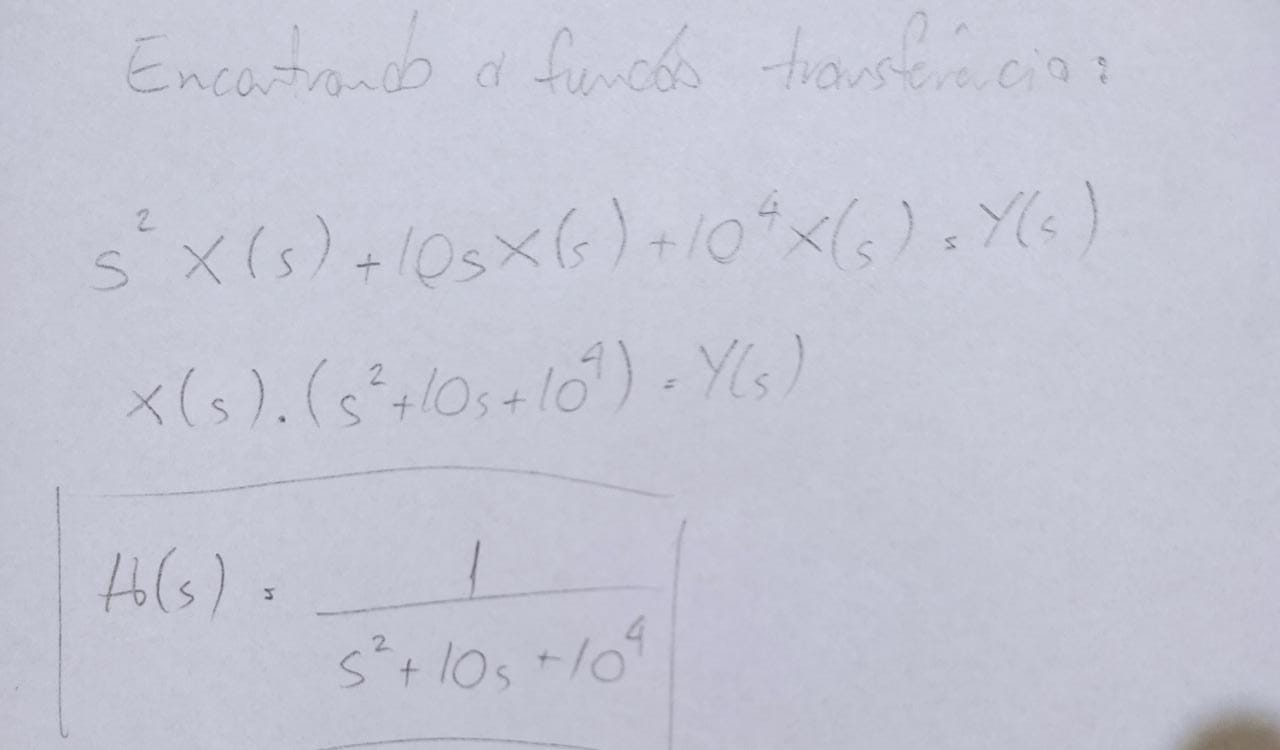
\includegraphics[scale=0.3]{imagens/a.jpg}
		\caption{Função Transferência}
	\end{figure}
	\begin{equation}
		H(s) = \frac{1}{s^2+10s+10^4}
	\end{equation}
	Com a função transferência podemos encontrar facilmente a FRF:
	\begin{equation}
		H(j\omega) = \frac{1}{(j\omega)^2+10\omega+10^4} = \frac{1}{-\omega^2 + 10j\omega + 10^4}
	\end{equation}
	
\section{Série de Fourier da Entrada}
	A entrada é um dente de serra com A = 100 e T = 0.1. Aplicando a série de Fourier temos:
	\begin{figure}[h]
		\center
		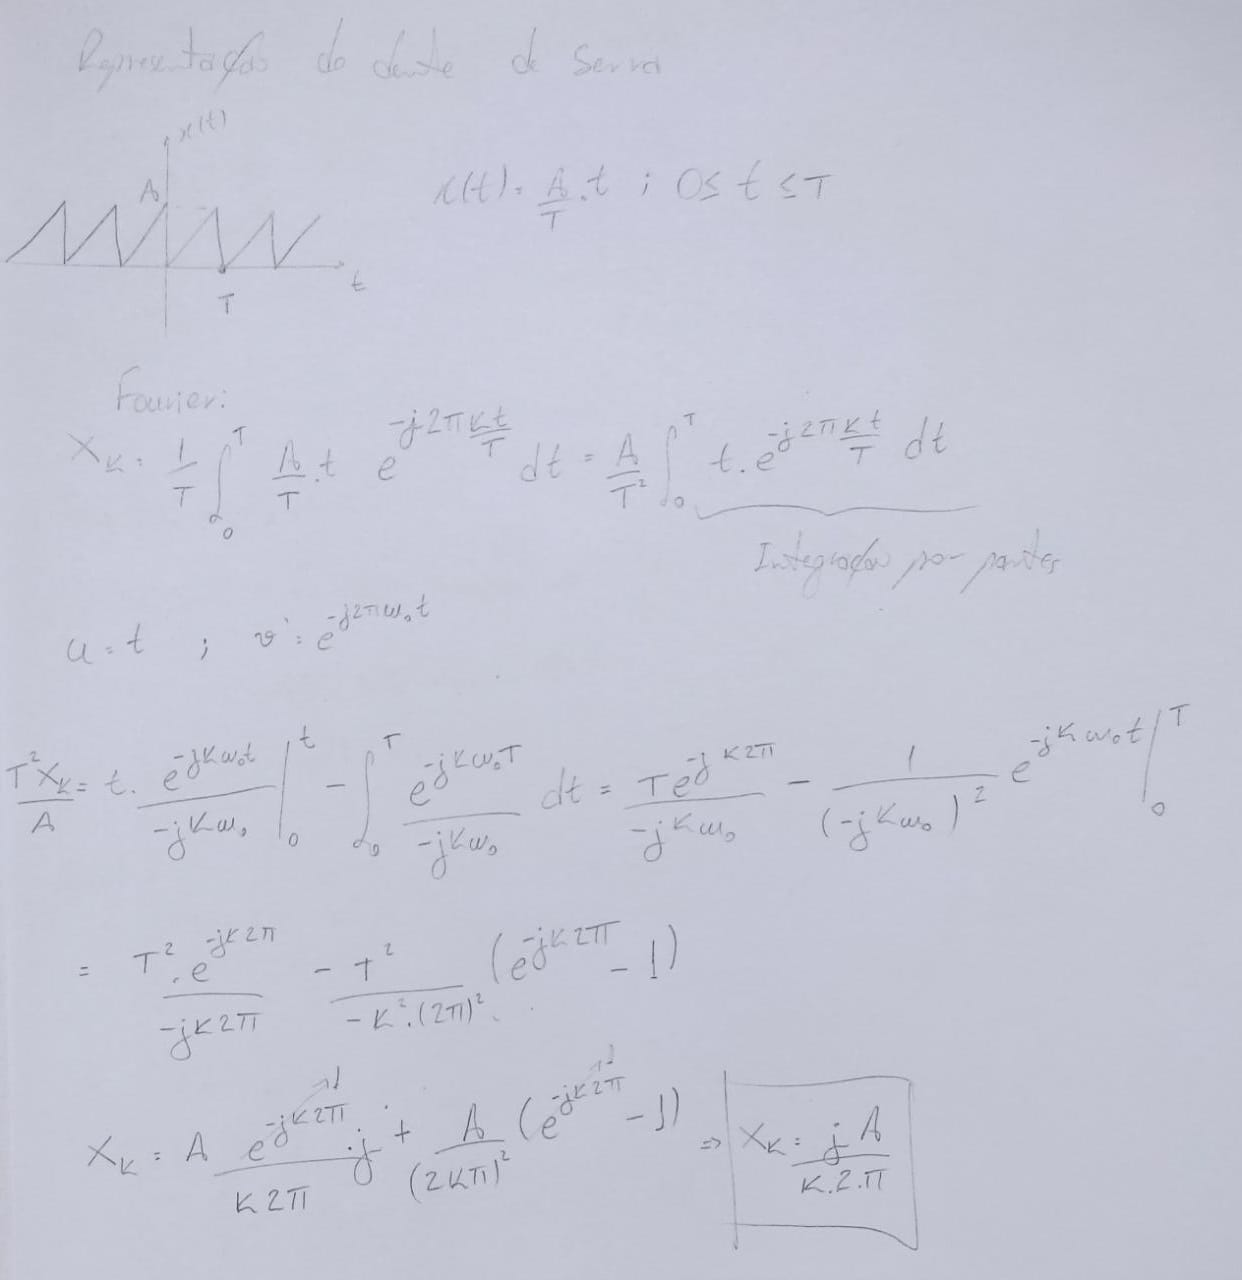
\includegraphics[scale=0.3]{imagens/aa.jpg}
		\caption{Série de Fourier do dente de serra}
	\end{figure}
	\begin{equation}
		X_k = \frac{j100}{k2\pi}
	\end{equation}		
	
\newpage
\section{Matlab}
	\subsection{Entrada}
		Plotando o gráfico da entrada temos:
		\begin{figure}[h]
			\center
			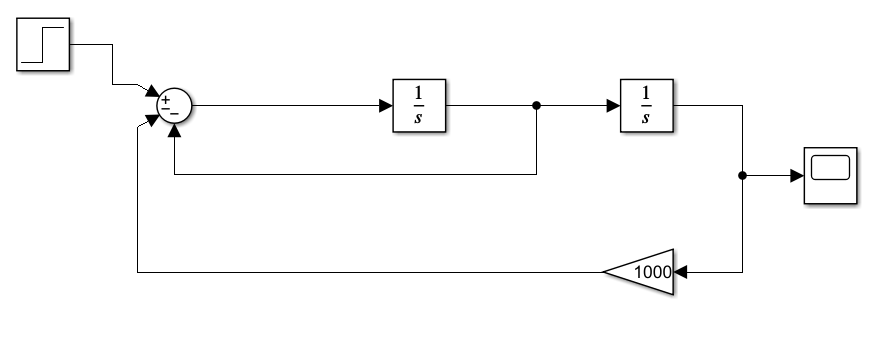
\includegraphics[scale=0.6]{imagens/aaa.png}
			\caption{Gráfico Série de Fourier do dente de serra}
		\end{figure}
	\subsection{Função resposta em frequência}
		Plotando o gráfico da FRF temos:
		\begin{figure}[h]
			\center
			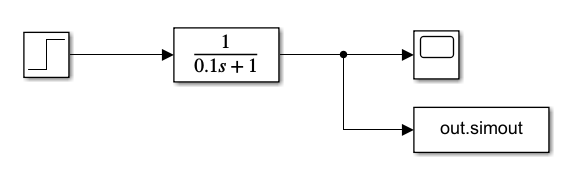
\includegraphics[scale=0.6]{imagens/aaaa.png}
			\caption{Gráfico FRF}
		\end{figure}
	\subsection{Resposta}
		Plotando o gráfico da resposta na frequência temos:
		\begin{figure}[h]
			\center
			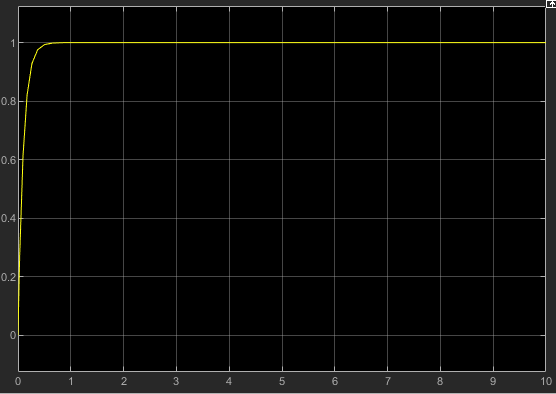
\includegraphics[scale=0.6]{imagens/aaaaa.png}
			\caption{Gráfico Resposta na frequência}
		\end{figure}

\section{Simulink}
	\begin{figure}[h]
		\center
		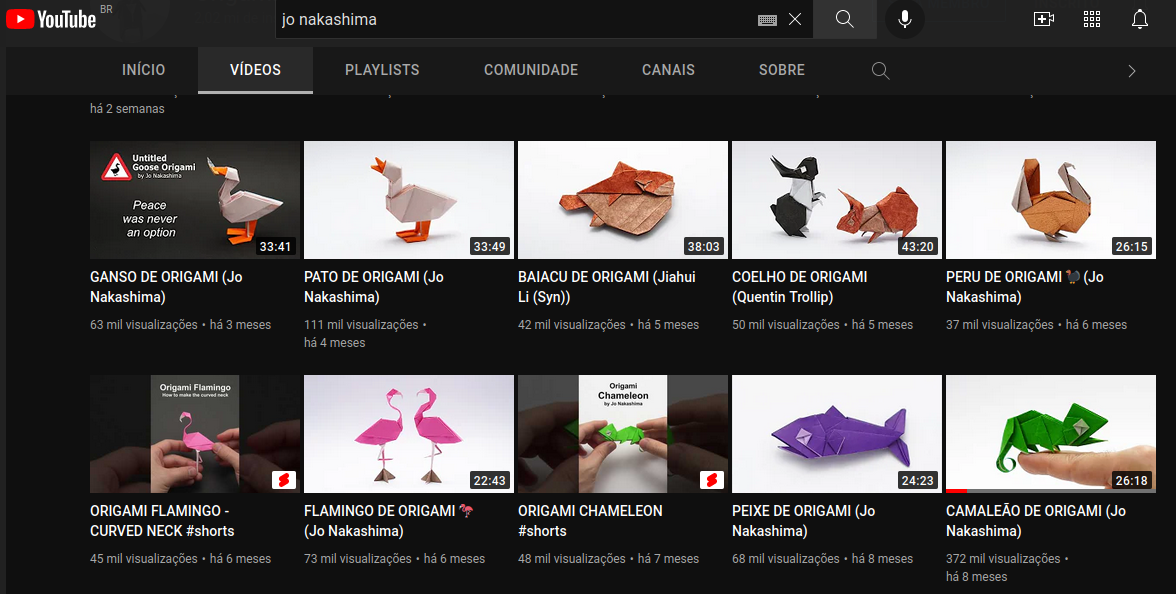
\includegraphics[scale=0.6]{imagens/b.png}
		\caption{Diagrama de Blocos}
	\end{figure}
	\subsection{Dente de Serra}
		Para aplicar o dente de serra no diagrama de blocos utilizamos o \textit{Signal Generator}, junto com os blocos de somador e a constante.\\
	\begin{figure}[h]
		\center
		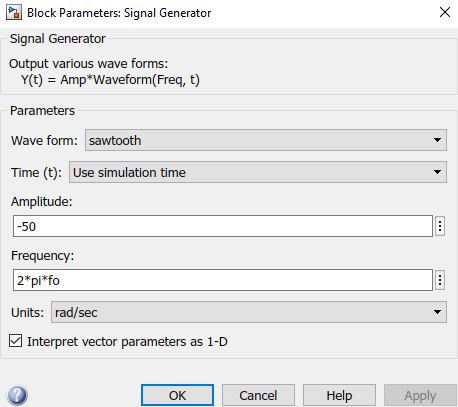
\includegraphics[scale=0.6]{imagens/bb.png}
		\caption{Configurações do Signal Generator}
	\end{figure}
	Como resultado temos o seguinte:
	\begin{figure}[h]
		\center
		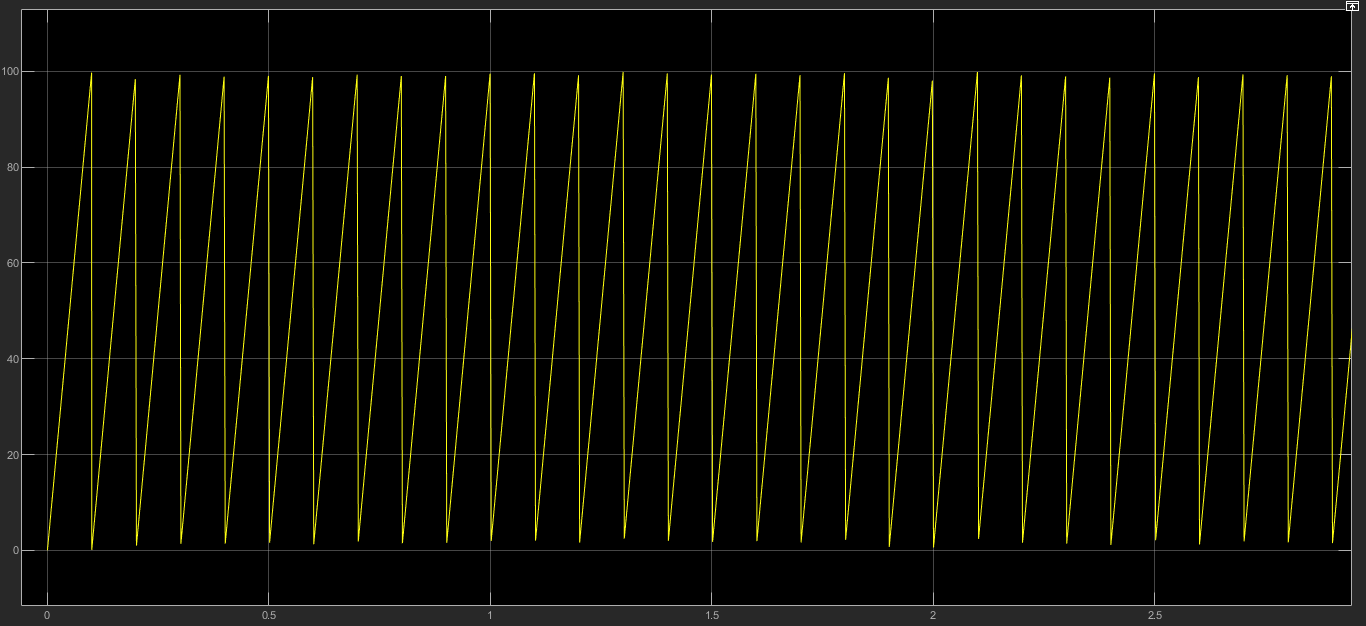
\includegraphics[scale=0.4]{imagens/bbb.png}
		\caption{Dente de Serra no simulink}
	\end{figure}
	\newpage
	Note que, o simulink não está plotando um gráfico com \textit{exatamente} 100 de amplitude. Isso pode ser um problema futuramente ao comparar a resposta forçada.
	
	\subsection{Saída do Escope}
	Depois de executar a simulação o Scope apresenta a seguinte resposta para o dente de serra:
	\begin{figure}[h]
		\center
		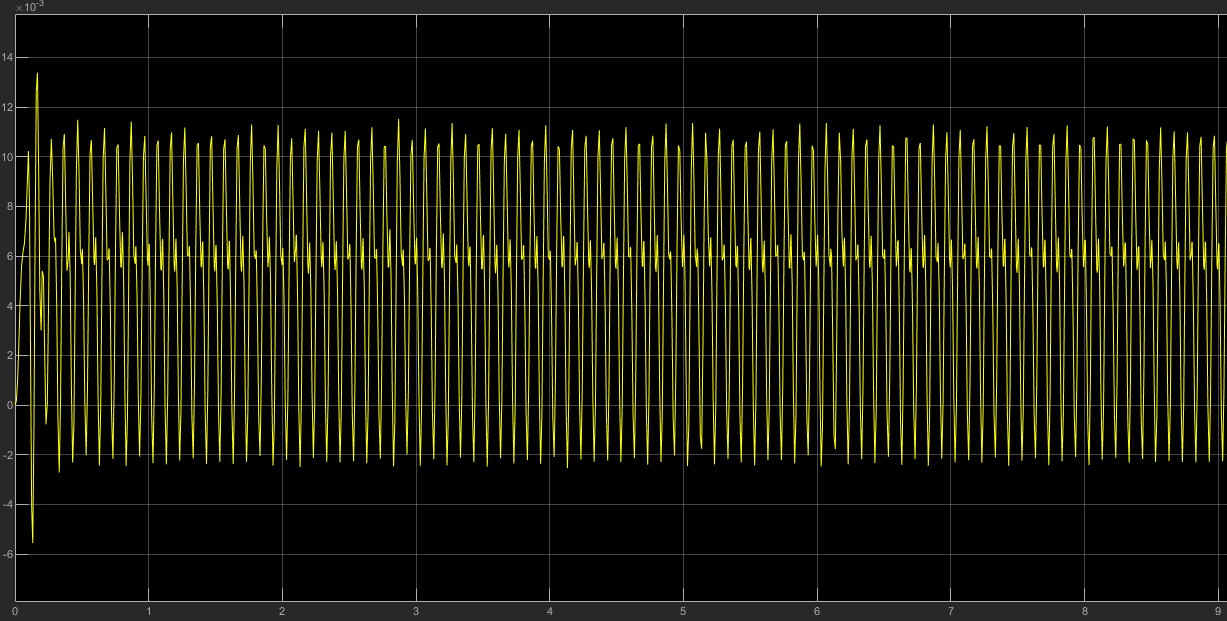
\includegraphics[scale=0.4]{imagens/bbbb.png}
		\caption{Resposta do Simulink}
	\end{figure}
	
	\subsection{Comparando Série de Fourier e Simulink}
	Anteriormente calculamos a \textit{resposta na freqûencia} por meio de Fourier. Para visualizar o resultado em função do tempo usamos a seguinte relação:
		\begin{equation}
			y(t) = y(t) + Y(k)e^{j2\pi k fo t}
		\end{equation}
	Plotando os dois resultados para a resposta ao dente de serra:\\
	\begin{figure}[h]
		\center
		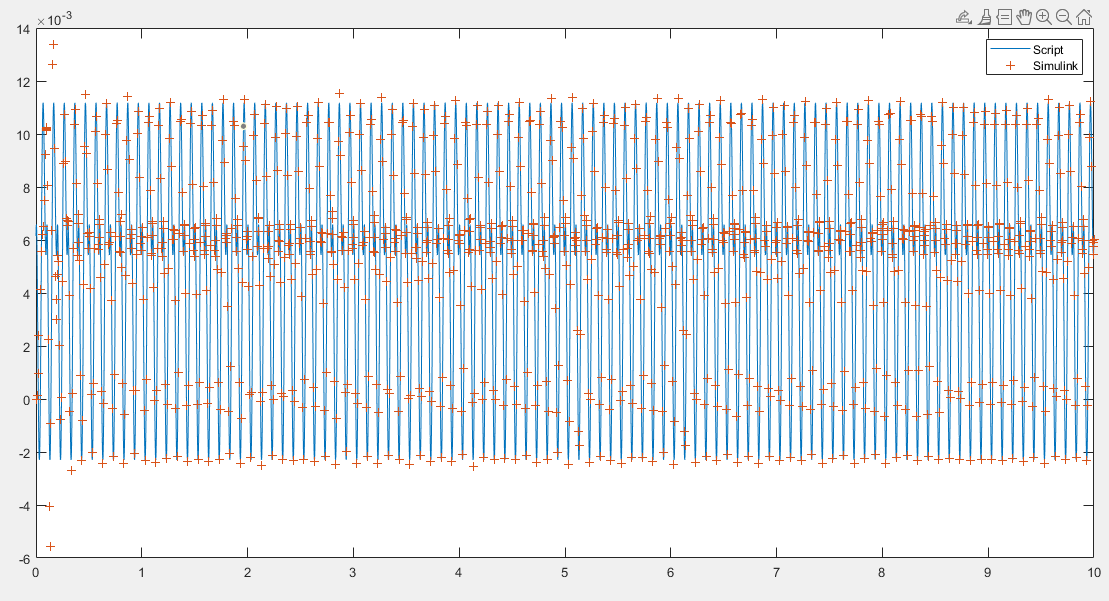
\includegraphics[scale=0.5]{imagens/bbbbb.png}
		\caption{Resposta do Simulink e por Série de Fourier}
	\end{figure}
	\newpage
	Veja que, em alguns pontos próximos ao vale e à crista da resposta os valores divergem. Isso ocorre pois 
a amplitude do dente de serra no simulink não possui exatamente amplitude 100.
	Com exceção desta observação, todos os pontos coincidem.
	
\newpage
\section{Código do Matlab}
	\begin{figure}[h]
		\center
		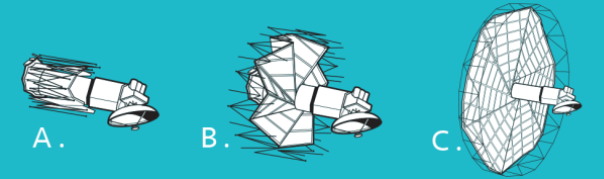
\includegraphics[scale=0.7]{imagens/c.png}
	\end{figure}
	\begin{figure}[h]
		\center
		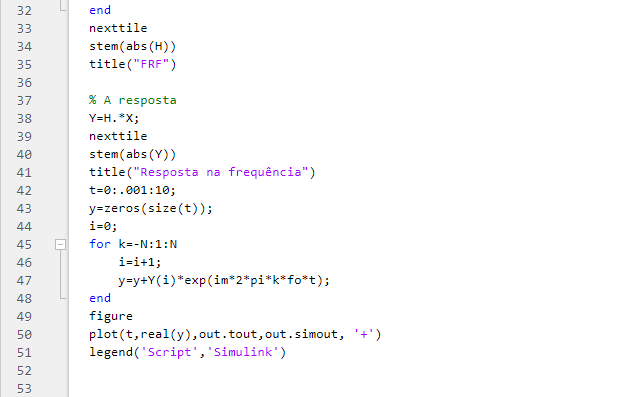
\includegraphics[scale=0.7]{imagens/cc.png}
		\caption{Código}
	\end{figure}
	
	
	
	
	
\end{document}